\section{A historical context of coherence theory}

The history of coherence theory is an intricate and fascinating tale rooted in
mathematics, statistics and physics, branching in classical and quantum directions with
profound implications for our understanding of the world. To tell it, we must go back to
the dawn of probability theory, where the idea of measuring relations between events and
variables first took shape --- a concept that, over the centuries, would evolve into the
refined notions of correlation and, eventually, coherence as we understand it today.

It all began in the seventeenth century, when thinkers such as Blaise Pascal and Pierre
de Fermat, in their correspondence on games of chance, laid the foundations of
probability theory. Their reflections on expected value and combinatorics opened the way
to Jacob Bernoulli, who in 1713, in his posthumous \textit{Ars Conjectandi}
\cite{bernoulli1713}, formulated the law of large numbers, linking theoretical
probability with observed frequency. These advances were consolidated by Pierre-Simon
Laplace in 1812 with his \textit{Théorie Analytique des Probabilités}
\cite{laplace1812theorie}, where he unified scattered ideas and developed Bayesian
inference, essential for understanding how variables relate in complex systems. Yet a
mathematical language was still missing to quantify the interdependence between phenomena.

That language began to take form in the nineteenth century. Carl Friedrich Gauss, in his
1809 study of errors in astronomical observations (\textit{Theoria Motus})
\cite{gauss1809theoria}, introduced the method of least squares, a tool that not only
optimised measurements but also revealed hidden patterns in correlated data. But it was
Francis Galton, in the 1880s, who coined the term ``correlation'' as we know it.
Motivated by his studies of biological inheritance, Galton sought to measure how
characteristics such as the height of parents and children varied together
\cite{galton1888correlations}. His work inspired Karl Pearson, who in 1896 formalised the
Pearson correlation coefficient \cite{pearson1896regression}, a number between $-1$ and
$1$ quantifying the linear relationship between variables. This was a conceptual leap: no
longer merely intuiting connections, but assigning them a rigorous numerical value.

In parallel, in the realm of physics, another kind of correlation --- coherence --- began
to reveal itself through the study of light. In 1801 Thomas Young performed his celebrated
double-slit experiment, showing that light interferes with itself, creating patterns of
bright and dark fringes. This phenomenon, inexplicable under Newton's corpuscular theory,
suggested that light was a wave whose phases could be correlated in space and time.
Augustin-Jean Fresnel, between 1815 and 1820, developed a mathematical theory of light as
a transverse wave, explaining not only interference but also polarisation. Coherence ---
the ability of waves to maintain a constant phase relationship --- was, however, not yet
understood in statistical terms.

The crucial step came in the first decades of the twentieth century, when optics met the
need to describe realistic light sources, such as the Sun or incandescent lamps, whose
emissions are partly random. In 1934 the Dutch physicist Pieter Hendrik van Cittert
published a seminal work on the propagation of coherence from an incoherent source
\cite{vancittert1934}, followed in 1938 by Frits Zernike \cite{zernike1938}, who
formulated the theorem that bears both their names: the \textbf{van Cittert--Zernike
theorem}. This result established that the light from an extended, incoherent source
develops measurable spatial correlations as it propagates to a distant plane. It was the
first time coherence had been quantified mathematically as a statistical property of
optical fields.

Classical coherence theory reached maturity in the 1950s through Max Born and Emil Wolf,
whose treatise \textit{Principles of Optics} (1959) \cite{born1999principles} became the
bible of theoretical optics. In it they defined the \textbf{mutual coherence function}

\begin{equation}
	\Gamma(\mathbf{r}_1, \mathbf{r}_2, \tau),
\end{equation}

which measures the correlation between the electric field at two points in space
($\mathbf{r}_1$ and $\mathbf{r}_2$) at two instants separated by a delay $\tau$. This
function encapsulates both the temporal coherence (how long the light maintains a stable
phase, related to its monochromaticity) and the spatial coherence (how correlated the
vibrations are at different positions). Leonard Mandel and Emil Wolf, in the following
decades, deepened these ideas in their treatise \textit{Optical Coherence and Quantum
Optics} \cite{mandel1995optical}, introducing concepts such as the coherence time and the
coherence length, key for practical applications.

Coherence was not a mere abstraction: the Michelson interferometer, developed in the
1890s, exploited temporal coherence to measure wavelengths with unprecedented precision.
But the technological milestone arrived in 1960 with the invention of the laser, whose
light --- highly coherent in time and space --- is the product of stimulated emission, a
phenomenon predicted by Einstein in 1917. Lasers not only confirmed the theories of
coherence but opened new frontiers in communications, medicine and industry.

While classical coherence was being consolidated, a parallel revolution was beginning in
the quantum world. In the 1960s quantum coherence found its theoretical framework. Roy J.
Glauber, in a series of articles published in \textit{Physical Review} (1963)
\cite{glauber1963quantum}, reformulated optics from a quantum perspective. He introduced
the \textbf{coherent states}, quantum analogues of classical waves with well-defined
phase, and defined the quantum correlation functions $g^{(n)}$, which measure the
probability of detecting several correlated photons. His work, awarded the Nobel Prize in
2005, not only explained phenomena such as photon antibunching but also laid the
foundations of modern quantum optics. The mathematical backbone connecting the statistical
description of fluctuations with their spectral content --- the
Wiener--Khinchin theorem \cite{wiener1930generalized,khinchin1934korrelationstheorie} ---
remains, as we shall see, one of the central pillars of the whole edifice.

In the twenty-first century, coherence has acquired a new flavour: the idea that it is a
quantifiable and exploitable \textbf{resource}, akin to energy or information
\cite{baumgratz2014quantifying}, integrated into the broader scheme of quantum computation.
In summary, the history of coherence is a journey from the abstract mathematics of
statistical correlations to the engineering of fragile quantum states. In its classical
guise it explains why stars twinkle, how lasers work and why holograms capture
three-dimensional images; in its quantum facet it challenges our intuition. And although
decoherence reminds us that these phenomena are ephemeral, it also underlines their value:
in a world where noise and chance seem to reign, coherence --- classical or quantum --- is
the thread that weaves order out of chaos.

\section{How is statistical similarity quantified?}

Suppose we have a completely random phenomenon --- such as the electromagnetic radiation
emitted by an incandescent bulb that is not in thermodynamic equilibrium, the number of
cars in some capital city throughout the day, the motion of an ion in a plasma, or
something as simple as throwing a ball into the air under non-ideal conditions.

When we wish to analyse statistically a single object or random variable, the familiar
tools appear: the probability density, the mean value, the standard deviation, the
kurtosis, and so on. What happens when we want to study at least two random variables and
how they relate? When we wish to study the statistics of two or more random variables we
must study the statistical similarity between them; but statistical similarity is a rather
broad concept, since we may have similarity in the mean values, or in the standard
deviations, or in the probability densities. To address this problem we return to linear
algebra.

If we have two vectors $\vec{A},\vec{B} \in \mathbb{R}^n$, the dot product
$\vec{A}\cdot\vec{B}$ is interpreted as the magnitude of the projection of $\vec{A}$ onto
$\vec{B}$ and vice versa; it can also be read as \textit{how much of $\vec{A}$ lies along
$\vec{B}$}. This behaviour can be extrapolated to continuous vector spaces, where one
usually employs the notion of inner product: if $f_A , f_B$ are two elements of a Hilbert
space $L^2$ of dimension $1$, one can define an inner product as

\begin{equation}\label{eq:ProdIn}
	\braket{f_A,f_B} = \int_\mathbb{R} f_A(x)f_B(x) W(x)\,dx,
\end{equation}

where $W(x)$ is some weight function.\footnote{$W(x)$ receives this name because, as it
says, it gives a weight to each value the integrand may take; there are no uniform
contributions, but rather each possible value of the integrand within the domain
contributes weighted by the value of $W$ at that point.} The interpretation is still
valid: this can be read as how much the function $f_A$ over all the reals coincides with
the function $f_B$ over all the reals.

To reach the notion of correlation from linear algebra we use a bit of bra--ket notation,
where the ket $\ket{f_A}$ represents a vector of an arbitrary Hilbert space $L^2$ and the
bra $\bra{f_A}$ represents an element of the dual of the same Hilbert space,\footnote{The
Hilbert space is a particular case of the $L^p$ spaces, the space of $p$-norm
Lebesgue-integrable functionals; for Hilbert $p=2$, and it has the property that the dual
of $L^2$ is also $L^2$, which lets quantum mechanics arise naturally in this space.} and
the inner product between them $\braket{f_A,f_A}= \braket{f_A|f_A}$ equals the probability
density of finding $f_A$ in a state $q \pm \triangle q$, where $q$ represents some
generalised coordinate. Suppose that $f_A,f_B \in L^2$ have the form

\begin{equation}
	\ket{f_A} = \hat{A}\ket{\Psi_A}, \quad \ket{f_B} = \hat{B}\ket{\Psi_B},
\end{equation}

where $\hat{A},\hat{B}$ are the operators of the physical quantities of
$\ket{\Psi_A},\ket{\Psi_B}$, so that we may interpret $\ket{f_A},\ket{f_B}$ as the wave
functions steered by their expected value. Using the inner product \eqref{eq:ProdIn} with
negligible weight function, the inner product reads

\begin{equation}
	\braket{f_A | f_B} = \int_{\mathbb{R^n}} \hat{A}\hat{B} \braket{\Psi_A|\Psi_B} d^nq = \int_{\mathbb{R^n}} \hat{A}\hat{B} P(A;B) d^nq,
\end{equation}

where we see that the similarity between $\ket{f_A}$ and $\ket{f_B}$ can be viewed as the
product of $\hat{A}$ with $\hat{B}$ times the probability density of having states $A$ and
$B$; that is, the similarity, or how \textit{correlated} two variables are, can be seen as
the integral of the product of the variables times their joint probability density.

With this analogy in mind we can understand correlation as a first measure of the
similarity between one or more variables across space and time. If $x_1(\vec{r},t_1),
x_2(\vec{r}',t_2)$ are two random variables and $p_2(x_2,t';x_1,t)$ is the joint
probability density, then the correlation between $x_1,x_2$ is defined as

\begin{equation}\label{eq:CorrFunc}
	\Gamma(\vec{r},\vec{r}';t_1,t_2) = E\left\{ x_1(\vec{r},t_1) x_2(\vec{r}',t_2)\right\},
\end{equation}

that is, as the ensemble average of $x_1\cdot x_2$.

\section{The coherence function}

The concept of the coherence function is, at the mathematical level, identical to that of
the correlation function given in equation \eqref{eq:CorrFunc}; both represent
correlations. However, coherence is a term widely used in the study of electromagnetic
radiation; let us see a little of why this is so.

\begin{figure}[htbp]
	\centering
	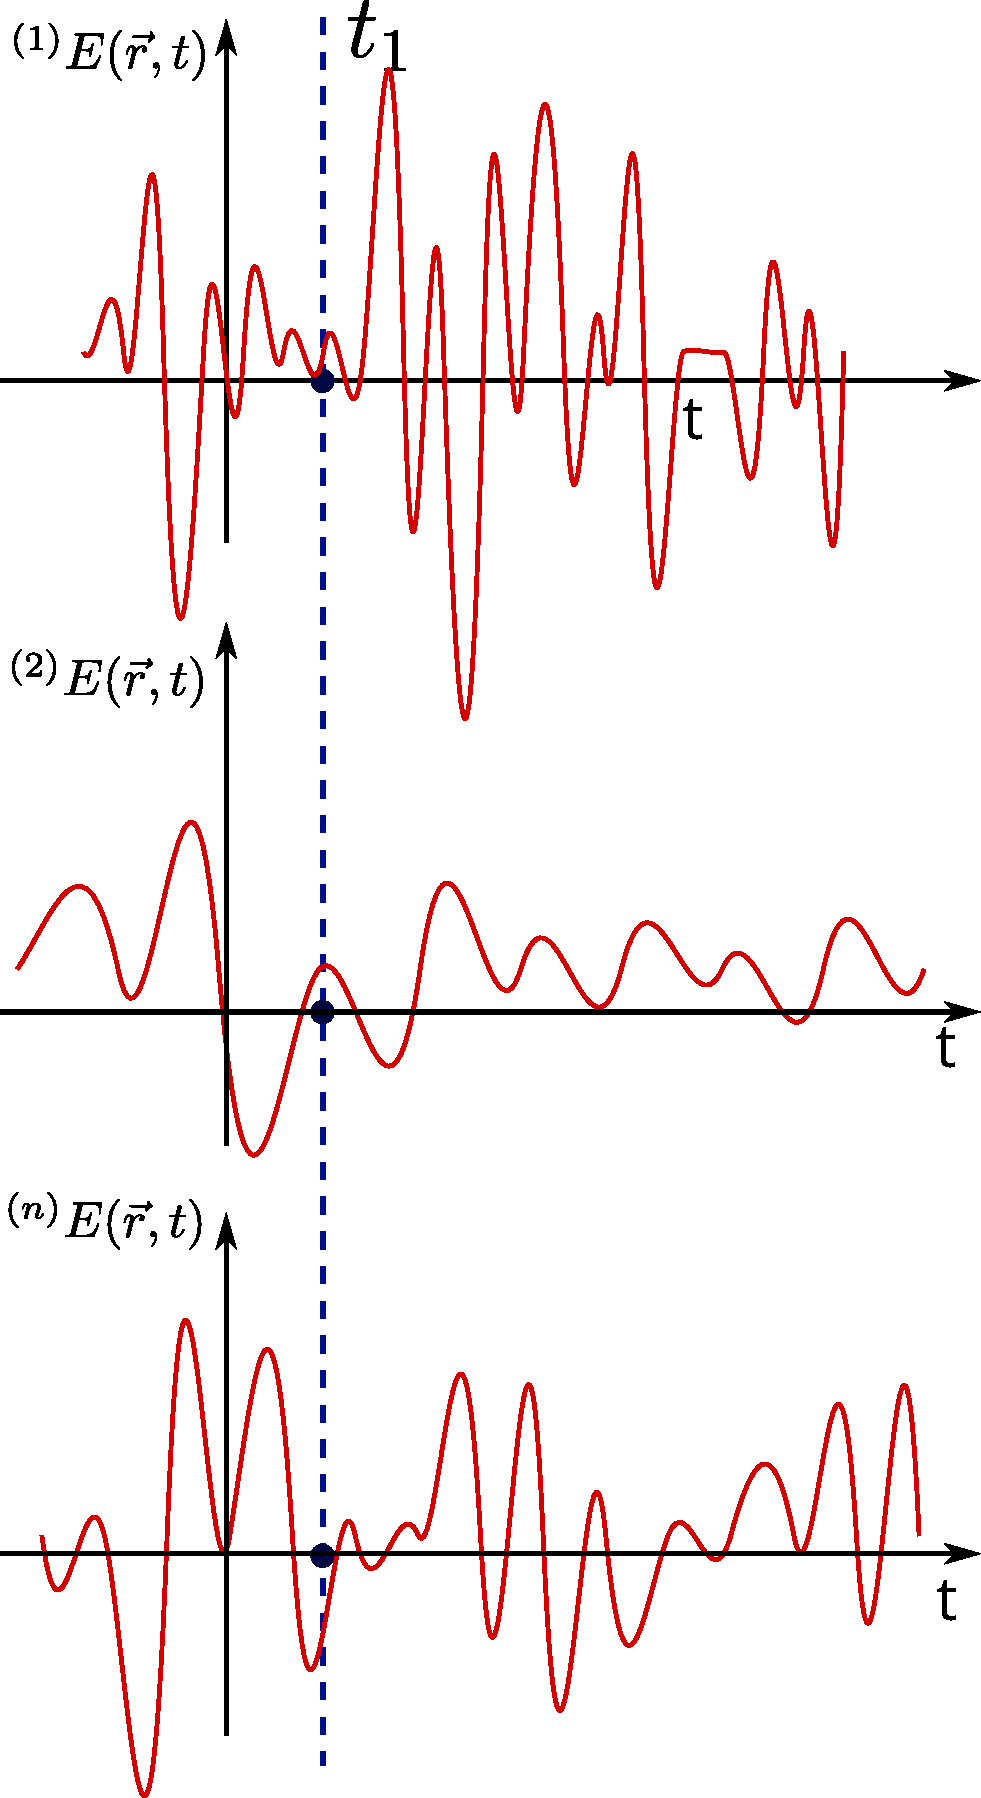
\includegraphics[width=0.4\linewidth]{Chapter 6/Figures/RandomVar}
	\caption{Representation of $E(\vec{r},t)$ as a random variable.}
	\label{fig:randomvar}
\end{figure}

In Figure~\ref{fig:randomvar} we observe a component of the electric field, represented by
$E(\vec{r},t)$, seen across several observations or realisations. Behaving as a random
variable, in each realisation it has a different behaviour in time at a point $\vec{r}$;
in general, here we have indexed $^{(i)}E(\vec{r},t)$ with integers, but in general there
could be an uncountable set of possible states for the electric field. If we look at
Figure~\ref{fig:randomvar} there are two temporal points, $t,t'$, at which we isolate
parts of these random oscillations; we could ask how correlated these oscillations are
across the realisations over the interval $t'-t$, or in other words, how
\textit{coherent} the oscillations are across the realisations.

We speak of coherence when we want to analyse the correlation of electromagnetic radiation
between space--time points. If we have two sources emitting an electric field (for the
moment understood as scalar), their coherence function is given by

\begin{equation}
	\Gamma(\vec{r},\vec{r}';t,t') = E \left\{ \mathcal{E} (\vec{r},t) \mathcal{E}^*(\vec{r}',t') \right\},
\end{equation}

where we are computing the ensemble average of the components $\mathcal{E}$, which are
complex numbers as already discussed in these notes. If we take $\vec{r}=\vec{r}'$ we
obtain what is known as the \textit{mutual coherence function}

\begin{equation}
	\Gamma(\vec{r}';t,t') = E \left\{ \mathcal{E}(\vec{r}',t) \mathcal{E}^*(\vec{r}',t') \right\}.
\end{equation}

We can go even further by including the concept of \textit{statistical stationarity}, but
one must be careful since there are several kinds. Formally, a stochastic process
$\{X_t\}$ is considered stationary when its statistical properties are invariant under
time translations. This condition manifests in different degrees:

\begin{enumerate}
	\item \textbf{Strict (strong) stationarity}: the most demanding form of stationarity requires that all joint probability distributions be time-invariant:

	\begin{equation}
		F_X(x_{t_1+\tau}, \ldots, x_{t_k+\tau}) = F_X(x_{t_1}, \ldots, x_{t_k}) \quad \forall \tau, k, t_i,
	\end{equation}
	where $F_X$ is the joint distribution function. This implies that:
	\begin{itemize}
		\item all moments (mean, variance, skewness, etc.) are constant;
		\item the marginal distributions are identical at any instant;
		\item it is a sufficient but not necessary condition for ARMA models.
	\end{itemize}

	\item \textbf{Weak (second-order) stationarity}: more practical in applications, it only requires invariance of the first two moments:
	\begin{equation}
		\begin{cases}
			\mathbb{E}[X_t] = \mu \quad (\text{constant}) \quad \forall t \\
			\text{Var}(X_t) = \sigma^2 \quad (\text{constant}) \quad \forall t \\
			\text{Cov}(X_t, X_{t+h}) = \gamma(h) \quad (\text{depends only on } h, \text{ not on } t)
		\end{cases}
	\end{equation}
	This is the definition used in most econometric models (ARIMA, GARCH) and in the Wiener--Khinchin spectral analysis (which we shall use later).

	\item \textbf{Trend stationarity (deterministic stationarity)}: a non-stationary process that can be made stationary by removing deterministic components:
	\begin{equation}
		X_t = \alpha + \beta t + \epsilon_t,
	\end{equation}
	where $\epsilon_t$ is stationary. The non-stationarity here comes exclusively from the temporal trend $\beta t$.
\end{enumerate}

We shall use a hypothesis of strong stationarity (although weak stationarity often
suffices). In this spirit, if $\tau = t-t'$ we have

\begin{equation}
	\Gamma(\vec{r}',t,t') = \Gamma(\vec{r}',t-t') = \Gamma(\vec{r}',\tau).
\end{equation}

As we can see, the mutual coherence at a point $\vec{r}'$ under a stationarity hypothesis
gives rise to an explicit dependence on the time difference $\tau$ in the ensemble average.

It is worth asking: how necessary is it to analyse the ensemble average; why not take the
temporal average? Answering this is \textbf{very complicated}, since it touches on the
problem of \textit{ergodicity}. Ergodicity, in the sense of ergodic theory, requires that
a dynamical system satisfy that the temporal averages coincide with the spatial averages
for almost every initial condition. Its rigorous proof is highly non-trivial, to the point
that the problems for which ergodicity has been proven with mathematical rigour are few.

From a phenomenological standpoint we shall assume, from now on, an \textit{ergodic
hypothesis} in which electromagnetic radiation has a stationary and ergodic character.
Under these conditions the mutual coherence function coincides with the temporal average

\begin{equation}
	\Gamma(\vec{r}';t,t') = \int_{\mathbb{R}} \mathcal{E}(\vec{r}',t') \mathcal{E}^*(\vec{r}',t-t')\,dt'.
\end{equation}

The mutual coherence function has several properties, some of which are:

\begin{itemize}
	\item[a)] $\Gamma(\vec{r}',0) \geq 0$. This follows from the definition, since $\Gamma(\vec{r}',0) = \braket{|\mathcal{E}(\vec{r}')|^2}$, i.e.\ it corresponds to the intensity of the electric field and can only be zero when trivially the field is zero at every instant.

	\item[b)] $\Gamma(\vec{r}',-\tau) = \Gamma^*(\vec{r}',\tau)$. This is known as the \textit{Hermitian property} of the mutual coherence function, and follows from the fact that $\mathcal{E}(\vec{r}',t)$ is stationary, which allows arbitrary temporal translations from the origin. In this spirit,

	\begin{align}
		& \Gamma(\vec{r}',\tau) = \braket{\mathcal{E}(\vec{r}')\mathcal{E}^*(\vec{r}',t + \tau)} = \braket{\mathcal{E}(\vec{r}',t-\tau)\mathcal{E}^*(\vec{r}')} = \Gamma^*(\vec{r}',-\tau).
	\end{align}

	\item[c)] $|\Gamma(\vec{r}',\tau)| \leq \Gamma(\vec{r}',0)$. This property follows from the \textit{Cauchy--Schwarz inequality}

	\begin{equation}
		|\Gamma(\vec{r}',\tau)|^2 = | \braket{\mathcal{E}(\vec{r}')\mathcal{E}^*(\vec{r}',t+\tau)} |^2 \leq  \braket{\mathcal{E}(\vec{r}',t)\mathcal{E}^*(\vec{r}',t)} \braket{\mathcal{E}(\vec{r}',t+\tau)\mathcal{E}^*(\vec{r}',t+\tau)} = \Gamma^2(\vec{r}',0),
	\end{equation}

	which implies that $|\Gamma(\vec{r}',\tau)|$ can never exceed its initial value $\Gamma(\vec{r}',0)$. (This property is, let us recall, exclusive to the mutual coherence function; when we consider the coherence between two sources we will see that it is not satisfied --- on the contrary, it will increase.)

	\item[d)] $\Gamma(\vec{r}',\tau)$ is non-negative. We can see this from the definition through the following, rather obvious, inequality

	\begin{equation}
		\left\langle \left| \int_{T_1}^{T_2} f(t)\mathcal{E}(t)\,dt \right|^2\right\rangle \geq 0,
	\end{equation}
	where $f(t)$ is an arbitrary function and $T_1,T_2$ are arbitrary times. In this way we obtain the inequality

	\begin{equation}
		\int_{T_1}^{T_2}\int_{T_1}^{T_2} f^*(\vec{r}',t)f(\vec{r}',t')\Gamma(\vec{r}',t'-t)\,dt\,dt' \geq 0.
	\end{equation}

	\item[e)] If the electric field is random, stationary and differentiable, then we can find a velocity $\xi (\vec{r}',t) = \dot{\mathcal{E}}(\vec{r}',t)$, which is stationary, random and of zero mean value, and whose mutual coherence function is

	\begin{equation}
		\Gamma_\xi(\vec{r}',\tau) = - \ddot{\Gamma}_\mathcal{E}(\vec{r}',\tau).
	\end{equation}

	\item[f)] $\Gamma(\vec{r}',\tau)$ is continuous. This holds even when there are jump discontinuities.
\end{itemize}

Finally, it is worth mentioning that there is a quantity known as the complex degree of
coherence, given by

\begin{equation}
	\gamma (\vec{r}',\tau) = \frac{\Gamma(\vec{r}',\tau)}{\Gamma(\vec{r}',0)},
\end{equation}

and from the Cauchy--Schwarz inequality we have $0 \leq |\gamma(\vec{r}',\tau)| \leq 1$.

\subsection{Manifestations of coherence: the Wiener--Khinchin theorem}

The mutual coherence function and the power spectral density are two sides of the same coin
in the study of light and wave signals. Mutual coherence describes how the fluctuations of
a luminous field are correlated in space and time, acting as a map that reveals to what
extent the variations at one point of space are synchronised with those at another, even
with a certain temporal delay. The power spectral density, in turn, decomposes the energy
of the signal into its frequency components, showing which tones or colours --- in the case
of light --- dominate its behaviour. The intimate relation between the two concepts lies in
the fact that, through mathematical transformations, it is possible to convert the detailed
information on the space--time correlations captured by mutual coherence into a precise
description of how the energy is distributed in the frequency domain, and vice versa. This
link allows researchers to jump between complementary perspectives: analysing interference
patterns in an interferometer or identifying spectral signatures in a material, all from
the same fundamental principles.

We are going to find one of the most important theorems in coherence theory, the
\textit{Wiener--Khinchin theorem}. Note that stationary random signals do not have a
Fourier transform; hence we may define the following truncated random signals of the
electric field

\begin{equation}\label{eq:NearlyWiener}
	^\omega \mathcal{E}_T (\vec{r},t) = \left\{
	\begin{matrix}
		^\omega\mathcal{E}(\vec{r},t) & -\frac{T}{2}\leq t \leq \frac{T}{2}\\
		0 & \text{otherwise}
	\end{matrix} \right.
\end{equation}

and we define the spectral power for a realisation $\omega$ as the squared magnitude of
the Fourier transforms of the electric fields \eqref{eq:NearlyWiener}, that is,

\begin{equation}\label{eq:SpecWT}
	^\omega S_T (\vec{r},\nu) = \left| \int_\mathbb{R} ^\omega \mathcal{E}_T(\vec{r},t)e^{i2\pi\nu t}dt \right|^2 = \left| \int_{-T/2}^{T/2}\;^\omega \mathcal{E}(\vec{r},t)e^{i2\pi\nu t}dt \right|^2,
\end{equation}

and the \textit{power spectral density of the event} $\omega$ we compute as

\begin{equation}\label{eq:SpecW}
	\lim_{T \to \infty} \frac{^\omega S_T(\vec{r},\nu)}{T} = {}^\omega S(\vec{r},\nu).
\end{equation}

Since we already possess a tool to study, in each event or realisation, the power spectral
density, then, through its ensemble average, we can find the total density, that is,

\begin{equation}
	S(\vec{r},\nu) = E\left\{^\omega S(\vec{r},\nu)\right\},
\end{equation}

introducing equations \eqref{eq:SpecWT} and \eqref{eq:SpecW} we then have

\begin{align}
	& S(\vec{r},\nu) = E\left\{ \lim_{T \to \infty} \left| \frac{1}{T} \int_{-T/2}^{T/2}\;^\omega \mathcal{E}(\vec{r},t)e^{i2\pi\nu t}dt \right|^2 \right\},\\
	& S(\vec{r},\nu) = \lim_{T \to \infty} \frac{1}{T}  \int_{-T/2}^{T/2}\int_{-T/2}^{T/2} E \left\{ \mathcal{E}(\vec{r},t)\mathcal{E}^*(\vec{r}',t') \right\} e^{i2\pi\nu(t-t')}dt\,dt',\\
	& S(\vec{r},\nu) = \int_{\mathbb{R}}\Gamma(\vec{r},\vec{r}';\tau)e^{i2\pi\nu \tau}d\tau,
\end{align}

\begin{equation}\label{eq:WienerKhinchin}
	\boxed{S(\vec{r},\nu) = \mathcal{F}\left\{ \Gamma(\vec{r},\vec{r}',\tau) \right\}}.
\end{equation}

Result \eqref{eq:WienerKhinchin} reads: the Fourier transform of the coherence function
corresponds to the power spectral density, and is known as the Wiener--Khinchin theorem.
Its use is fundamental, since it tells us that by methods such as spectrometry we can find
the coherence function of any phenomenon; we can even go further, since this result really
stems from something more general --- the correlation function --- meaning that every
stochastic phenomenon has an associated spectrum, and from the measurements or estimates of
that spectrum we can compute the correlations in the system.

If we make a simple observation, the optical range of radiation --- the visible --- is a
band of very low frequencies relative to the whole spectrum; the visible runs roughly from
$400$~nm to $700$~nm, and we may say that all of optics is \textit{narrowband}. This obeys
the inequality

\begin{equation}
	\frac{\triangle \nu}{\nu} \ll 1,
\end{equation}

and, in this narrowband regime, the coherence function takes the form

\begin{equation}
	\Gamma(\vec{r};\tau) = \tilde{\Gamma}(\vec{r})e^{i2\pi \tilde{\nu}\tau},
\end{equation}

which we can represent graphically as shown in Figure~\ref{fig:narrow}, where one can see
the behaviour of the coherence function in the narrowband regime.\footnote{One usually
finds in the literature a term similar but not equal to that of narrowband, known as the
quasi-monochromaticity condition, written as $\frac{\triangle \lambda}{\lambda} \ll 1$; but
this bounds the wavelength so that it is as monochromatic as possible, while the narrowband
condition admits several frequencies, provided they are narrow relative to the whole
frequency spectrum.} There one sees an envelope (the observable) enveloping all the
fundamental frequencies.

\begin{figure}[htbp]
	\centering
	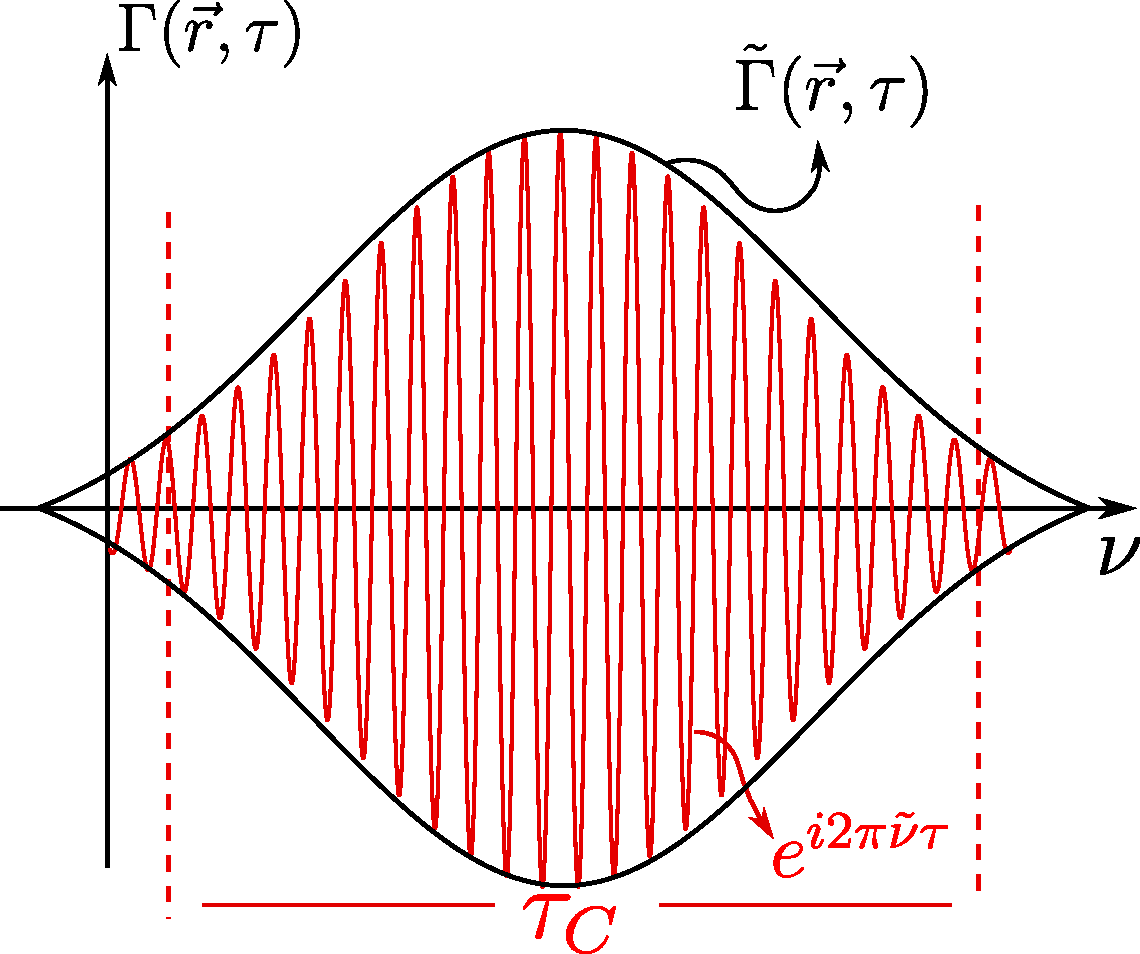
\includegraphics[width=0.7\linewidth]{Chapter 6/Figures/Estrecho}
	\caption{Graphical representation of the narrowband coherence function. In black, the envelope $\tilde{\Gamma}(\vec{r},\tau)$ is shown, and in red the oscillations $e^{i2\pi\tilde{\nu}\tau}$. These oscillations are confined within something known as the coherence time $\tau_C$, which we shall see later.}
	\label{fig:narrow}
\end{figure}

\subsection{The wave equation of coherence}

Let us step a little out of the comfort zone and understand how correlations propagate
through space and time. Let $\mathcal{E}^{(r)}(\vec{r},t)$ be some \textbf{real} component
of the electric field, viewed as a random signal. As is well known from classical
electromagnetic theory, it obeys Maxwell's equations and therefore has an associated wave
equation, namely

\begin{equation}
	\nabla^2 \mathcal{E}^{(r)}(\vec{r},t) = \frac{1}{C^2}\frac{\partial^2 \mathcal{E}^{(r)}(\vec{r},t)}{\partial t^2},
\end{equation}

where $C$ is the speed of light in vacuum. We also have, by Fourier analysis,

\begin{equation}\label{eq:EandFourier}
	\mathcal{E}(\vec{r},t) = \int_0^{\infty} \tilde{\mathcal{E}}(\vec{r},\nu) e^{-i2\pi\nu t}d\nu .
\end{equation}

And if we apply the d'Alembertian operator $\square = \nabla^2 -
\frac{1}{C^2}\frac{\partial^2}{\partial t^2}$ to equation \eqref{eq:EandFourier}, we find
that $\tilde{\mathcal{E}}(\vec{r},\nu)$ has the form of a Helmholtz-type equation, that is,

\begin{equation}
	\nabla^2 \mathcal{E}(\vec{r},t) - \frac{1}{C^2}\frac{\partial^2 \mathcal{E}(\vec{r},t)}{\partial t^2} = \int_0^{\infty} \left[ \nabla^2 \tilde{\mathcal{E}}(\vec{r},\nu) + k^2 \tilde{\mathcal{E}}(\vec{r},\nu) \right]e^{-i2\pi\nu t}d\nu,
\end{equation}

which leads us to the fact that the electric field, as an analytic and complex signal, also
obeys a wave-type equation

\begin{equation}
	\nabla^2 \mathcal{E}(\vec{r},t) = \frac{1}{C^2}\frac{\partial^2 \mathcal{E}(\vec{r},t)}{\partial t^2}.
\end{equation}

Taking the complex conjugate of the previous equation we have

\begin{equation}\label{eq:NearlyWaveForE}
	\nabla^2 \mathcal{E}^*(\vec{r},t) = \frac{1}{C^2}\frac{\partial^2 \mathcal{E}^*(\vec{r},t)}{\partial t^2}.
\end{equation}

If we multiply both sides of equation \eqref{eq:NearlyWaveForE} by
$\mathcal{E}(\vec{r}',t')$, and since we have taken the d'Alembertian with respect to the
unprimed variables, using some sign rules we have

\begin{equation}\label{eq:NoAvg}
	\nabla^2 \left[ \mathcal{E}^*(\vec{r},t)\mathcal{E}(\vec{r}',t') \right] =  \frac{1}{C^2} \frac{\partial^2}{\partial t^2}\left[ \mathcal{E}^*(\vec{r},t)\mathcal{E}(\vec{r}',t') \right].
\end{equation}

Taking the ensemble average of equation \eqref{eq:NoAvg} over all realisations of the
field, this wave equation becomes

\begin{equation}\label{eq:coherenceWave1}
	\nabla^2 \Gamma(\vec{r},\vec{r}';t,t') = \frac{1}{C^2}\frac{\partial^2}{\partial t^2} \Gamma(\vec{r},\vec{r}';t,t'),
\end{equation}

and, similarly, using $\square' = \nabla'^2 - \frac{1}{C^2}\frac{\partial^2}{\partial t'^2}$
we have another wave equation given by

\begin{equation}\label{eq:coherenceWave2}
	\nabla'^2 \Gamma(\vec{r},\vec{r}';t,t') = \frac{1}{C^2}\frac{\partial^2}{\partial t'^2} \Gamma(\vec{r},\vec{r}';t,t').
\end{equation}

Equations \eqref{eq:coherenceWave1} and \eqref{eq:coherenceWave2} tell us directly that the
coherence functions between two space--time points evolve in time following a wave-type
equation, separately, with respect to each pair of space--time coordinates --- a result
that is, without doubt, remarkable. We can take this result even further and study this
propagation in the next section.

\subsection{Propagation of coherence and the direction of time: the van Cittert--Zernike theorem}

\begin{figure}[htbp]
	\centering
	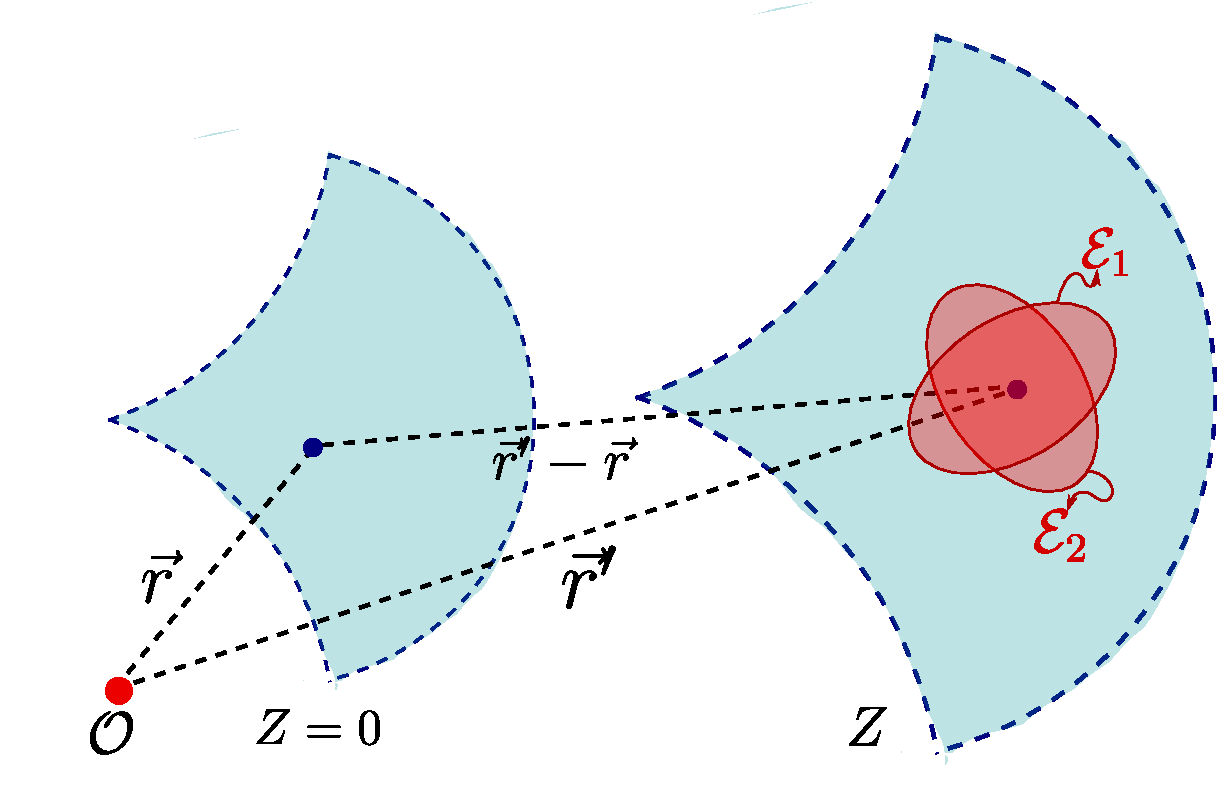
\includegraphics[width=0.8\linewidth]{Chapter 6/Figures/Propagation}
	\caption{Propagation of the electric field from a plane $Z=0$ to a plane $Z$, where each point of the wavefront carries its mean polarisation ellipse.}
	\label{fig:propagation}
\end{figure}

As we know, the electric field obeys a wave-type equation and the orientation of the
fields is given by the polarisation of the field; in turn, as we saw in the diffraction
chapter (see Section~\ref{Sec:Diffraction}), at the classical level light fundamentally
propagates as spherical waves, as illustrated in Figure~\ref{fig:propagation}, and at each
point of the wavefront the components of the electric field oscillate randomly, but within
the mean polarisation ellipse of their representative state. Mathematically we can
represent this component as

\begin{equation}
	\mathcal{E}_z(\vec{r}_1,\nu) = \frac{i}{\lambda} \int_{\Sigma} \mathcal{E}_0 (\vec{r},\nu) \frac{e^{ik \|\vec{r}_1-\vec{r}\|}}{\|\vec{r}_1-\vec{r}\|}\cos(\hat{z}; \vec{r}_1-\vec{r})\,d\sigma .
\end{equation}

Using equation \eqref{eq:EandFourier} we have

\begin{equation}
	\mathcal{E}_z(\vec{r}_1,t) = \frac{1}{i}\int_{\mathbb{R}^+} \frac{\nu}{V} \int_{\Sigma} \mathcal{E}_0(\vec{r},\nu)\frac{\cos\left(  \hat{z}; \vec{r}_1 - \vec{r} \right)}{\|\vec{r}_1 - \vec{r}\|} e^{i2\pi \nu \left( t + \frac{\|\vec{r}_1 - \vec{r}\|}{V} \right)} d\sigma\, d\nu,
\end{equation}

where $V$ is the propagation velocity of the envelope. Rewriting a little more, we have

\begin{equation}
	\mathcal{E}_z(\vec{r}_1,t) = \frac{1}{i} \int_{\Sigma} \frac{\cos\left( \hat{z}; \vec{r}_1-\vec{r} \right)}{\|\vec{r}_1 -\vec{r}\|} \int _{\mathbb{R}^+} \frac{\nu}{V} \mathcal{E}_0 (\vec{r},\nu)e^{i2\pi\nu \left(t + \frac{\|\vec{r}_1 - \vec{r}\|}{V}\right)}d\nu\, d\sigma,
\end{equation}

and, taking the narrowband approximation, we have

\begin{equation}\label{eq:IntegralEz}
	\mathcal{E}_z(\vec{r}_1,t) = \frac{1}{i\tilde{\lambda}} \int_{\Sigma} \mathcal{E}_0 \left(\vec{r}, t +\frac{\|\vec{r}_1 - \vec{r}\|}{V}\right) \frac{\cos\left(\hat{z} ; \vec{r}_1 - \vec{r}\right)}{\|\vec{r}_1-\vec{r}\|} d\sigma .
\end{equation}

We can visualise graphically how we intend to propagate in Figure~\ref{fig:propagation2},
where we observe that we are starting from the coherence function between two points
$\vec{r},\vec{r}'$ at instants $t,t'$, respectively, and carrying it to a coherence function
at the points $\vec{r}_1,\vec{r}_2$ at two instants $t_1,t_2$, respectively.

\begin{figure}[htbp]
	\centering
	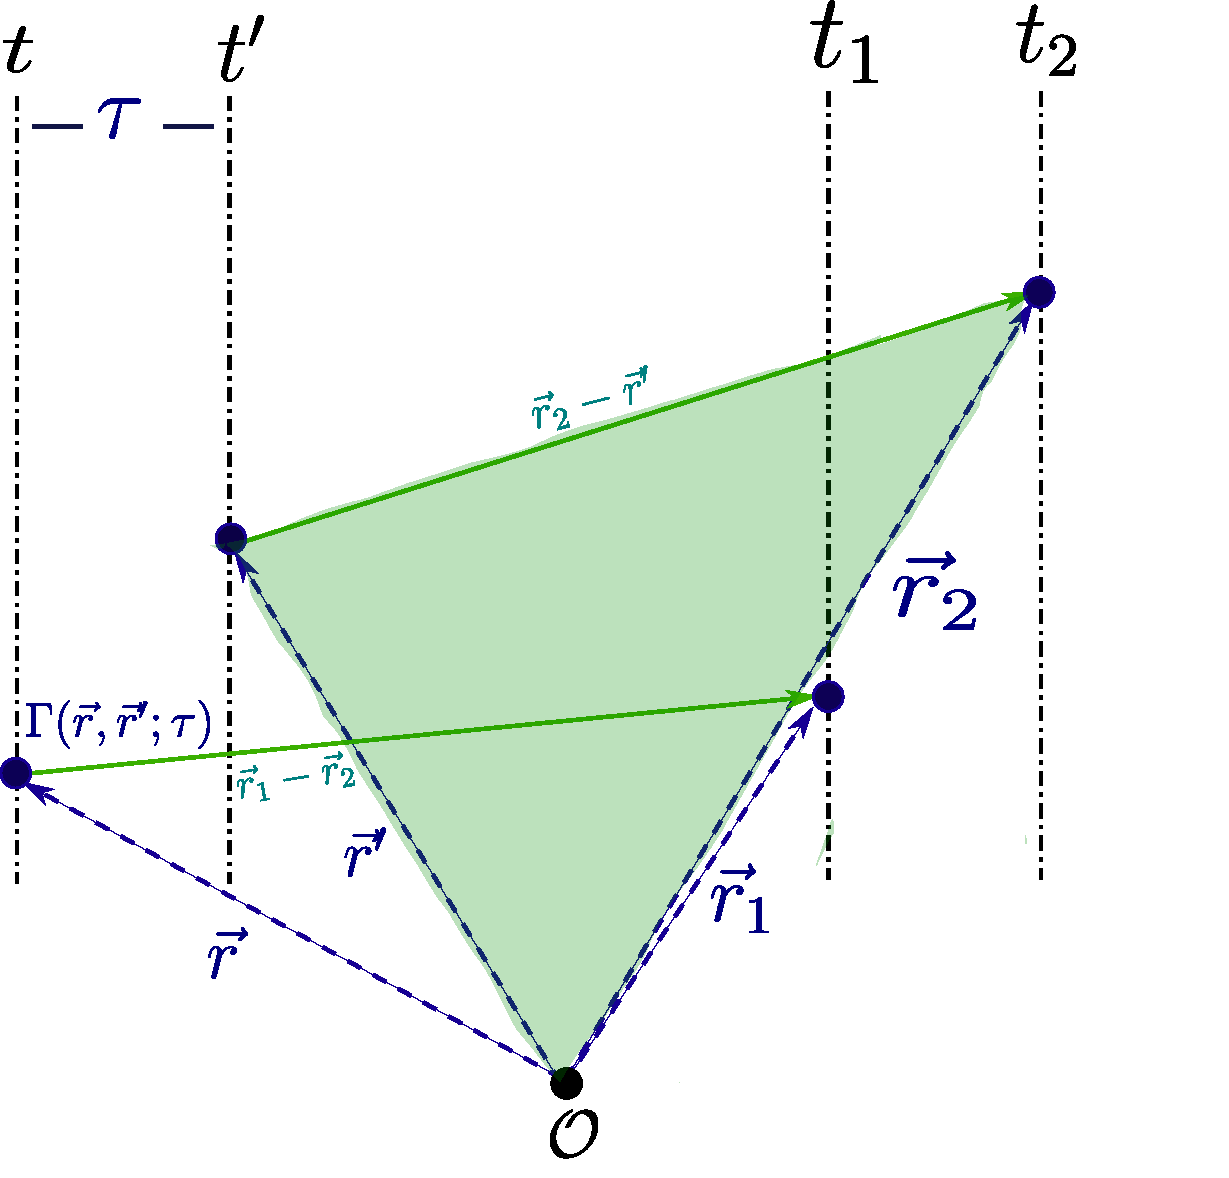
\includegraphics[width=0.8\linewidth]{Chapter 6/Figures/Propagation2}
	\caption{Propagation of the coherence function between two points $\vec{r},\vec{r}'$ on the initial plane to the coherence between two points $\vec{r}_1,\vec{r}_2$ on the observation plane.}
	\label{fig:propagation2}
\end{figure}

Starting from equation \eqref{eq:IntegralEz} we can compute the coherence function in its
propagation as

\begin{equation}
	\Gamma_z(\vec{r}_1,\vec{r}_2;\tau) = E \left\{ \mathcal{E}_z(\vec{r}_1,t) \mathcal{E}_z^*(\vec{r}_2,t-\tau) \right\},
\end{equation}

\begin{align}
	&\Gamma_z(\vec{r}_1,\vec{r}_2;\tau) = E\left\{\frac{1}{i\tilde{\lambda}} \int_{\Sigma} \mathcal{E}_0 \left(\vec{r},t + \frac{\|\vec{r}_1 - \vec{r}\|}{V}\right) \frac{\cos\left(\hat{z};\vec{r}_1-\vec{r}\right)}{\|\vec{r}_1-\vec{r}\|}d\sigma \right. \\
	& \left. \cdot \frac{1}{-i\tilde{\lambda}} \int_{\Sigma'} \mathcal{E}_0^* \left(\vec{r}',t - \tau + \frac{\|\vec{r}_2 - \vec{r}'\|}{V}\right) \frac{\cos\left(\hat{z};\vec{r}_2-\vec{r}'\right)}{\|\vec{r}_2-\vec{r}'\|}d\sigma'  \right\},
\end{align}

\begin{align}
	& \Gamma_z(\vec{r}_1,\vec{r}_2;\tau) = \frac{1}{\tilde{\lambda}^2} \int_{\Sigma}\int_{\Sigma'} E \left\{ \mathcal{E}_0\left(\vec{r}, t + \frac{\|\vec{r}_1 - \vec{r}\|}{V}\right) \mathcal{E}_0^* \left(\vec{r}', t-\tau + \frac{\|\vec{r}_2 - \vec{r}'\|}{V}\right) \right\}\frac{\cos \left(\hat{z};\vec{r}_1-\vec{r}\right) \cos\left(\hat{z}; \vec{r}_2 - \vec{r}' \right) }{\|\vec{r}_2-\vec{r}'\|\cdot \|\vec{r}_1 - \vec{r}\|} d\sigma\, d\sigma',
\end{align}

\begin{equation}\label{eq:IntGamma}
	\Gamma_z (\vec{r}_1,\vec{r}_2;\tau) = \frac{1}{\tilde{\lambda}^2}\int_{\Sigma}\int_{\Sigma'} \Gamma_0 \left(\vec{r},\vec{r}';\tau + \frac{\|\vec{r}_1 - \vec{r}\| + \|\vec{r}_2 - \vec{r}'\|}{V}\right) \frac{\cos \left(\hat{z};\vec{r}_1-\vec{r}\right) \cos\left(\hat{z}; \vec{r}_2 - \vec{r}' \right) }{\|\vec{r}_2-\vec{r}'\|\cdot \|\vec{r}_1 - \vec{r}\|} d\sigma\, d\sigma'
\end{equation}

\begin{figure}[htbp]
	\centering
	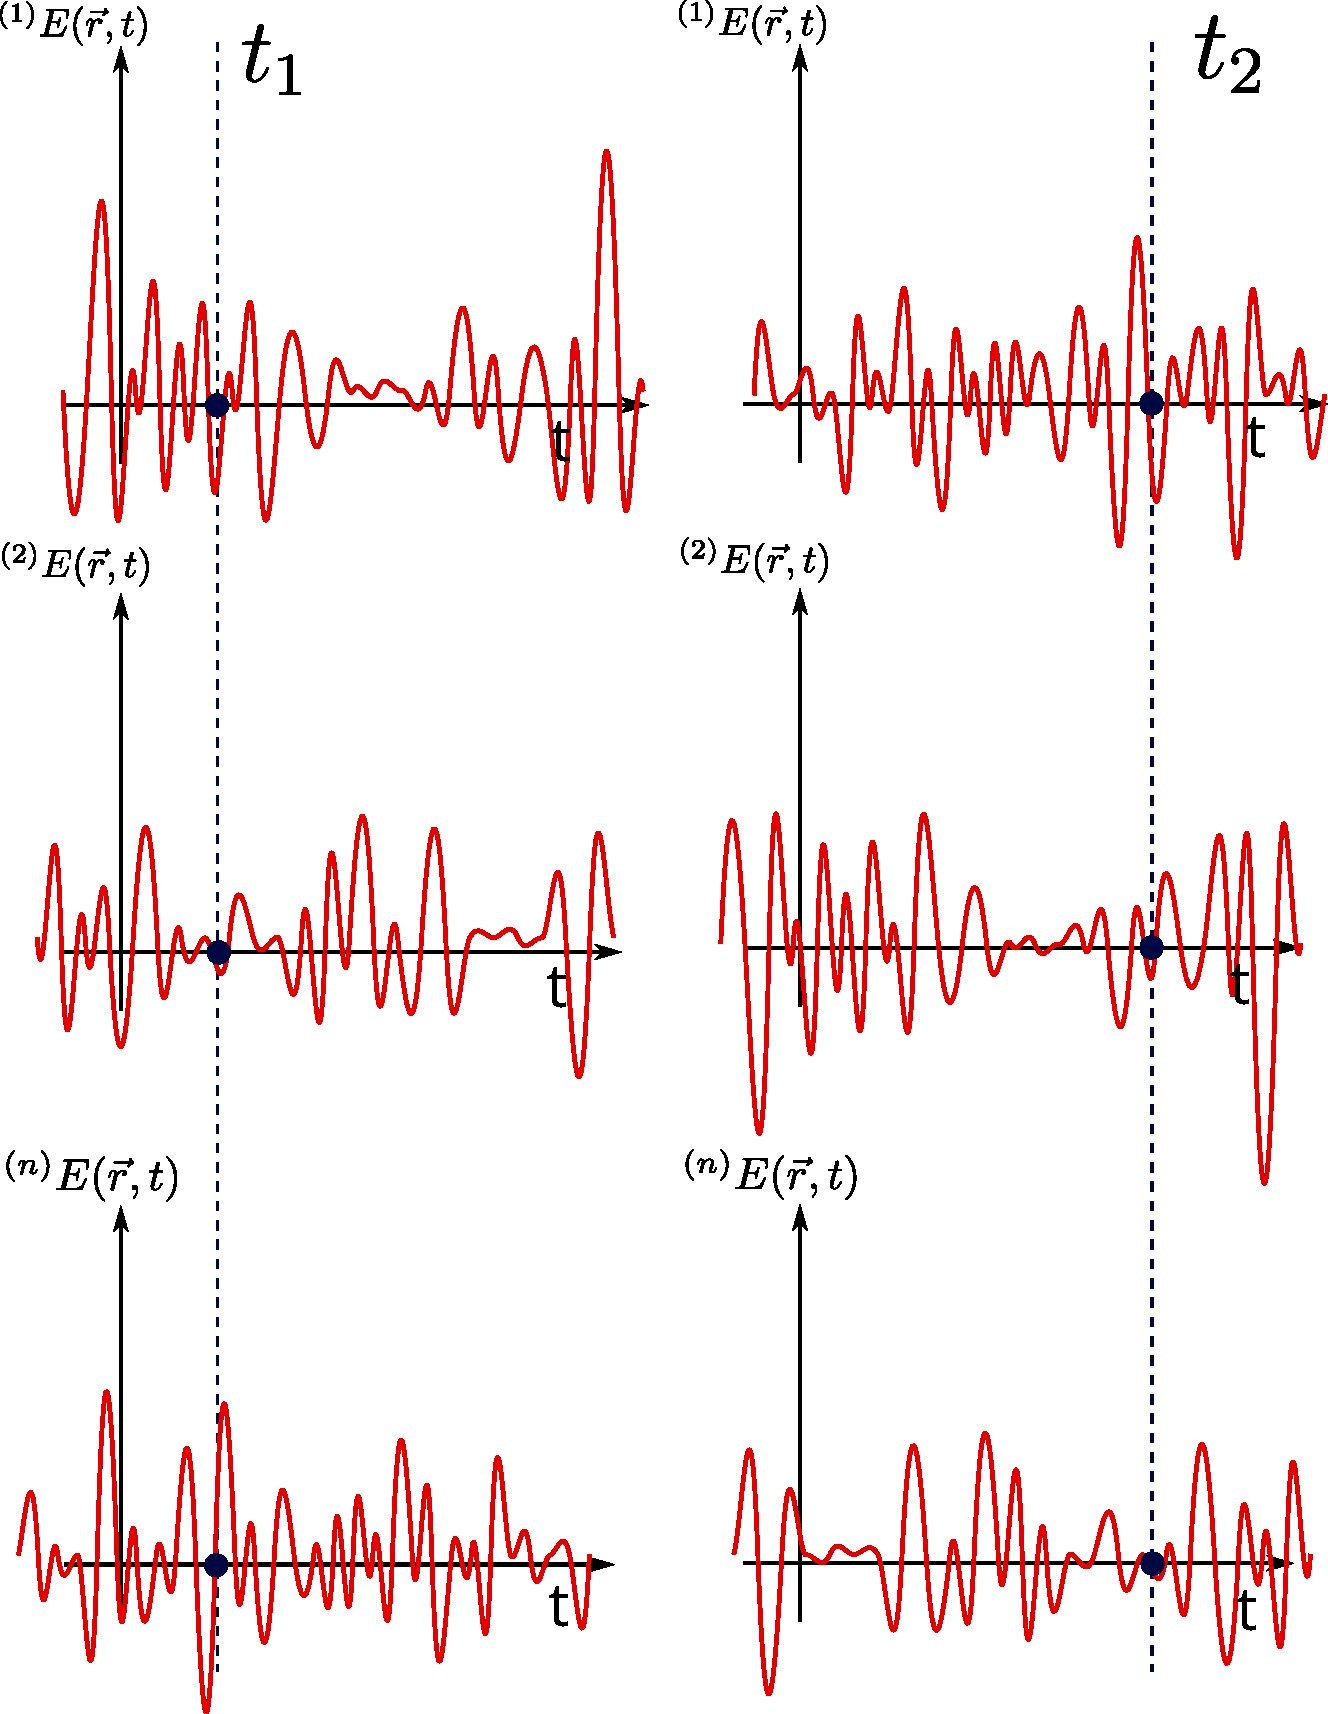
\includegraphics[width=0.6\linewidth]{Chapter 6/Figures/Random2}
	\caption{Evolution of the realisations upon propagating the electric field.}
	\label{fig:random2}
\end{figure}

The propagation of the random oscillations across $n$ realisations can be visualised in
Figure~\ref{fig:random2}.

We are going to impose the following condition on the coherence function

\begin{equation}
	\Gamma(\vec{r},\vec{r}';\tau) = \Gamma(\vec{r}';\tau) \delta(\vec{r}-\vec{r}'),
\end{equation}

which, in a few words, means that, spatially speaking, the distribution representing the
coherence function is point-localised and weighted by the mutual coherence at the point
$\vec{r}'$. Imposing this on equation \eqref{eq:IntGamma} we have

\begin{equation}
	\Gamma_z\left(\vec{r}_1,\vec{r}_2;\tau\right) = \frac{1}{\tilde{\lambda}^2}\int_{\Sigma}\Gamma_0 \left( \vec{r}; \tau + \frac{\|\vec{r}-\vec{r}_1\| - \|\vec{r} -\vec{r}_2\| }{V} \right)\frac{\cos \left(\hat{z};\vec{r}_1-\vec{r}\right) \cos\left(\hat{z}; \vec{r}_2 - \vec{r} \right) }{\|\vec{r}_2-\vec{r}\|\cdot \|\vec{r}_1 - \vec{r}\|} d\sigma .
\end{equation}

In nature we will not always have narrowband sources; however, we can resort to another
argument, namely that most instruments do not have an infinite or broad range but a short
one --- or, in other words, measurement instruments measure a narrow part of the spectrum.
Therefore, including the narrowband condition we have

\begin{equation}
	\Gamma_z(\vec{r}_1,\vec{r}_2)e^{i2\pi\tilde{\nu}\tau} = \frac{1}{\tilde{\lambda}^2} \int_{\Sigma} \Gamma_0(\vec{r})e^{i2\pi\tilde{\nu} \left( \tau + \frac{\|\vec{r} - \vec{r}_1\| - \|\vec{r}-\vec{r}_2\|}{V} \right) } \frac{\cos \left(\hat{z};\vec{r}_1-\vec{r}\right) \cos\left(\hat{z}; \vec{r}_2 - \vec{r} \right) }{\|\vec{r}_2-\vec{r}\|\cdot \|\vec{r}_1 - \vec{r}\|} d\sigma .
\end{equation}

Given the coherence time defined by $\tau_C = \int_{\mathbb{R}^+}| \gamma(\vec{r},\tau) |^2
d\tau$, and if we impose a condition of very small times, smaller than a coherence time
$\tau \ll \tau_C$, we have

\begin{equation}
	\Gamma_z(\vec{r}_1,\vec{r}_2) = \frac{1}{\tilde{\lambda}^2}\int_{\Sigma}I_0(\vec{r})e^{i2\pi \left( \frac{\|\vec{r}-\vec{r}_1\| - \|\vec{r} - \vec{r}_2\|}{V/\tilde{\nu}} \right)} \frac{\cos \left(\hat{z};\vec{r}_1-\vec{r}\right) \cos\left(\hat{z}; \vec{r}_2 - \vec{r} \right) }{\|\vec{r}_2-\vec{r}\|\cdot \|\vec{r}_1 - \vec{r}\|} d\sigma .
\end{equation}

Taking the far-field approximation we can simplify the problem as follows

\begin{equation}\label{eq:IntegralProx}
	\Gamma_z(\vec{r}_1,\vec{r}_2) = \frac{1}{\tilde{\lambda}^2 z^2} \int_{\Sigma} I_0(\vec{r}) e^{i2\pi \left( \frac{\|\vec{r}-\vec{r}_1\| - \|\vec{r} - \vec{r}_2\|}{V/\tilde{\nu}} \right)} d\sigma .
\end{equation}

We may now make a Taylor-series expansion, the same one performed in the diffraction
chapter. In this spirit the following terms become

\begin{align}
	& \|\vec{r} - \vec{r}_1\| = \left( z^2 + (x-x_1)^2 + (y-y_1)^2 \right)^{1/2} = z \left(1 + \frac{(x-x_1)^2 + (y-y_1)^2}{z^2}\right)^{1/2} \approx z + \frac{(x-x_1)^2 + (y-y_1)^2}{2z},\\
	& \|\vec{r}-\vec{r}_2\| \approx z + \frac{(x-x_2)^2 + (y-y_2)^2}{2z}.
\end{align}

Introducing this into integral \eqref{eq:IntegralProx} we obtain

\begin{equation}
	\Gamma_z (\vec{r}_1,\vec{r}_2) = \frac{1}{\tilde{\lambda}^2 z^2}\int_{\mathbb{R}^2}I_0(x,y)e^{-\frac{i2\pi}{\tilde{\lambda}z}\left(xx_1 + yy_1\right)}e^{\frac{i2\pi}{\tilde{\lambda} z}(xx_2 + yy_2)} e^{-\frac{i\pi}{\tilde{\lambda}z}(x_1^2 + y_1^2)}dx\,dy.
\end{equation}

Let us define the vectors $\vec{S}_1 = (x_1,y_1)$, $\vec{S}_2 = (x_2,y_2)$ and $\vec{S} =
(x,y)$. Then

\begin{equation}
	\Gamma_z(\vec{S}_1,\vec{S}_2) = \frac{e^{i \frac{\pi}{\tilde{\lambda}z} (\|\vec{S}_1\|^2 - \|\vec{S}_2\|^2)}}{\tilde{\lambda}^2 z^2} \int_{\mathbb{R}^2} I_0(\vec{S})e^{-i \frac{2\pi}{\tilde{\lambda}z}\vec{S}\cdot (\vec{S}_1 - \vec{S}_2)}dS.
\end{equation}

If we set $\vec{S}_2 = \vec{0}$ we arrive at the Fourier integral

\begin{equation}
	\boxed{ \Gamma_z (\vec{S}_1)  = \frac{e^{\frac{i\pi}{\tilde{\lambda}z}\|\vec{S}_1\|^2} }{\tilde{\lambda}^2z^2}\int_{\mathbb{R}^2} \Gamma_0(\vec{S}) e^{-\frac{i2\pi}{\tilde{\lambda}z}\vec{S}\cdot\vec{S}_1}dS},
\end{equation}

which, basically, means that the correlations, under all the approximations we have made,
propagate by means of a Fourier integral; or, what is the same, the van Cittert--Zernike
theorem tells us that coherence diffracts --- it propagates naturally as a diffraction
integral (see Figure~\ref{fig:fouriergamma}).

\begin{figure}[htbp]
	\centering
	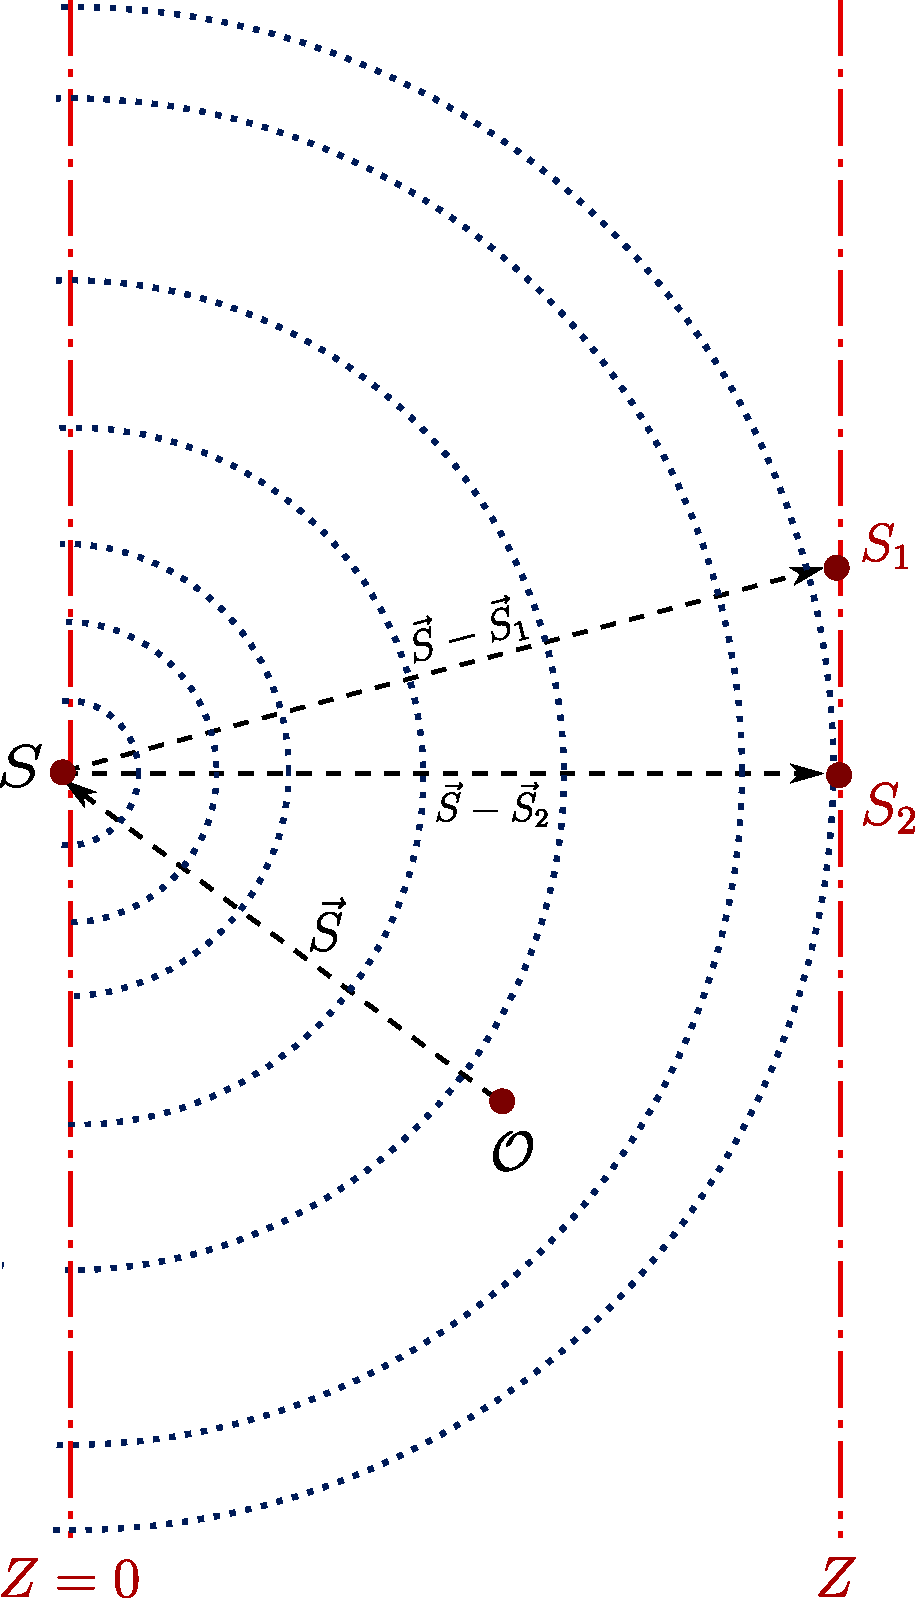
\includegraphics[width=0.65\linewidth]{Chapter 6/Figures/FourierGamma}
	\caption{The mutual coherence propagated to the far field is the Fourier transform of the intensity distribution $\Gamma_0(\vec{S})$ of the source.}
	\label{fig:fouriergamma}
\end{figure}

How can we tell in which direction time flows? This may sound like a question rather out of
context for these notes, but if we could travel back to the golden age of Boltzmann, we
would find a heated debate of the time on how statistical physics gives a direction to
time, an \textit{arrow}. Paraphrasing Boltzmann, it is said that \textit{time advances in
the direction in which correlations increase}. If we look at the van Cittert--Zernike
theorem, we can start from two completely uncorrelated sources but, as they propagate, they
gradually become correlated; time grows and so does coherence, until a point is reached at
which the radiation of those sources is coherent. This is, without doubt, one of the
strongest and most beautiful results we can find in statistical physics.
